\documentclass[oneside,final,14pt]{extreport}
\usepackage[utf8]{inputenc}
\usepackage[ukrainian]{babel}
\usepackage{vmargin}
%\usepackage{cmap}
\usepackage{siunitx,hyperref,lipsum}

\usepackage{nameref,zref-xr}
\zxrsetup{toltxlabel}

\DeclareUnicodeCharacter{00A0}{\nobreakspace}

\usepackage{amssymb,amsmath}

\usepackage[pdftex]{graphicx} 
\graphicspath{{../images1/}{../images/}}
\DeclareGraphicsExtensions{.pdf,.jpeg,.png,.jpg}

\usepackage{titlesec}
\titleformat{\chapter}
  {\normalfont\fontsize{14}{16}\bfseries\centering} % format
  {\thesection}  % label
  {1em}          % sep
  {}             % before-code
\titleformat{\section}
  {\normalfont\fontsize{14}{16}\bfseries} % format
  {\thesection}  % label
  {1em}          % sep
  {}             % before-code
\titleformat{\subsection}
  {\normalfont\fontsize{14}{14}} % format
  {}  % label
  {1em}          % sep
  {}             % before-code

\setpapersize{A4}
\setmarginsrb{2.5cm}{2cm}{1.5cm}{1cm}{0pt}{0mm}{0pt}{13mm}
\usepackage{indentfirst}
\sloppy

%\vspace{10pt}
%\addvspace{10pt}
%\setlength{\parskip}{7pt plus4mm minus3mm}
\usepackage{setspace} 
\onehalfspacing

%sub do_cmd_textasciitilde{ '~' . @_[0]; }
%sub do_cmd_textasciicircum{ '^' . @_[0]; }

\title{ПРОГРАМНИЙ МОДУЛЬ ВИЯВЛЕННЯ ЗАЛЕЖНОСТЕЙ МІЖ ПОТЕНЦІЙНО-НЕБЕЗПЕЧНИМИ ДЕФЕКТАМИ ПОЧАТКОВОГО ТЕКСТУ ЦІЛЬОВИХ ПРОГРАМ КІБЕРНЕТИЧНОГО ВПЛИВУ}
\author{Васильців А.А.}

\begin{document} % Маркер начала документа
\maketitle % Создать титульный лист на основе данных в заголовке документа

\chapter*{АНОТАЦІЯ}
\label{0annotation:annotation}
Кваліфікаційна робота бакалавра: 72  с., 12  рис., 2  таблиці, 2 додатки, 16 джерел.

Дана бакалаврська робота присвячена розробці модуля пошуку дефектів реакції програм. Даний модуль призначений для аналізу програмного коду на предмет вразливостей та оцінки рівня їх небезпечності. Цей модуль може використовуватись як у рамках  кафедри №21 ВІТІ НТУУ “КПІ”, так і за її межами у інформаційно-телекомунікаційних вузлах ЗСУ.

Модуль пошуку дефектів реакції програм  реалізований із застосуванням об’єктно-орієнтованої мови програмування  C ++, PHP, CMS Joomla, бібліотеки libExploit, генератора парсерів BISON, лексичного аналізатора FLEX, системи керування базами даних MySQL 

%TODO
ANNOTATION
\normalfont


Qualifying work degree: 72 p., 12 img., 2 table, 2 add, 16 sources.

This undergraduate paper is devoted to developing search module defect response programs. This module is designed to analyze the code in terms of vulnerabilities and assessment of their danger. This module can be used as part of the department number 21 VITI KPI and outside military headquarters in the UAF.

Search module defect response programs implemented using object-oriented programming language C ++, PHP, CMS Joomla, librarie libExploit, parser generator BISON, FLEX, database management system MySQL.
\pagebreak

\setcounter{tocdepth}{1}
\tableofcontents % Создать содержание документа (потребуется дважды сформировать документ для того,
% чтобы номера страниц сформировались правильно)
\newpage % Начать следующий раздел с новой страницы
\chapter*{ВСТУП}
\addcontentsline{toc}{chapter}{ВСТУП}
\label{1entrance::doc}\label{1entrance:id1}
Підготовка фахівців з нав’язування кібернетичного впливу та захисту вимагає напрацювання теоретичних знань і практичних навичок з використання інструментальних засобів дослідження потенційно-небезпечних дефектів реакції програм. На сьогодні існує низка засобів для здійснення аналізу та пошуку дефектів, та зазвичай вони є недостатньо інформативними та вимагають попередньої підготовки у використанні ними, тому існує необхідність у створенні більш інтерактивних, масштабованих та інформативних, що сприятиме процесу навчання. Актуальність роботи полягає у створенні програмно-технічних засобів пошуку та дослідження потенційно-небезпечних дефектів реакції програм.

Об’єкт дослідження – підготовка фахівців з аналізу та використання потенційно-небезпечних дефектів реакції програм.

Предмет дослідження – інструментальні засоби  аналізу та використання потенційно-небезпечних дефектів реакції програм.

Мета роботи: Розробити програмно-технічний комплекс для відпрацювання практичних навичок фахівців з аналізу та використання потенційно-небезпечних дефектів реакції програм щодо переповнення.
\begin{description}
\item[{Завдання:}] \leavevmode\begin{enumerate}
\item {} 
Проаналізувати напрямки підготовки фахівців з нав’язування кібернетичного впливу;

\item {} 
Побудувати програмно-технічний комплекс дослідження цільових програм на переповнення буфера;

\item {} 
Проаналізувати існуючі метрики програмного коду на предмет можливості використання їх для оцінки потенційно вразливих ділянок вихідних текстів програм

\item {} 
Провести оцінку цінності підготовки фахівців з нав’язування кібернетичного впливу на основі переповнення буферу.

\end{enumerate}

\end{description}
\pagebreak

\chapter{АНАЛІЗ МЕТОДОЛОГІЧНИХ ОСНОВ РОЗРОБКИ ЗАСОБІВ КІБЕРНЕТИЧНОГО ВПЛИВУ }
\label{1section::doc}\label{1section:id1}

%TODO на початку вказати на необхідність організації КА

\section{Організація, принципи розробки засобів кібернетичного впливу}
\label{1section:id2}
Виходячи зі змісту та ролі інформації у сучасному світі, американський дослідник М. Маклюен виводить цікаву тезу, що звучить так: ``Істинно тотальна війна - це війна за допомогою інформації''.
Аналіз сучасних поглядів дозволяє вважати, що інформаційна боротьба (ІБ) у цілому є комплексом взаємопов'язаних і узгоджених за цілями, місцем і часом заходів, орієнтованих на досягнення інформаційної переваги. Вона є результатом нових інформаційних технологій. У наслідок їх застосування набули змін не тільки засоби збройної боротьби, але й стратегія, і тактика ведення сучасних воєн, з'явилися нові концепції ведення бойових дій у ``інформаційному столітті'', що враховують нові фактори вразливості сторін.
Кібернетичний вплив – це сукупність дій, спрямованих на зміну порядку функціонування інформаційної системи. 
%вставити рисунок 

На сьогоднішній час інформаційні технології впроваджуються у сфери  діяльності людини. Не виключенням є військові організації, від рівня надійності яких напряму залежить національна безпека країни. Однак з стрімким розвитком виникає проблема захисту від комп'ютерних атак, техніка яких також постійно розвивається.
Зростання можливостей щодо несанкціонованого одержання інформації, а також зацікавлення у несанкціонованому одержанні інформації, поява додаткових каналів витоку інформації, передусім у процесі обробки інформації засобами електронно-обчислювальної техніки, використання нових методів і засобів несанкціонованого здобуття інформації значно ускладнили умови інформаційної безпеки, особливо в частині протидії технічній розвідці та попередження несанкціонованої модифікації інформації  шляхом зараження її вірусами і програмними  закладками різних видів і типів.

Забезпечення інформаційної безпеки в умовах, що постійно змінюються, вимагає постійного проведення:

\begin{itemize}
\item{прикладних досліджень явищ і процесів у даній предметній області, відповідно - підготовки фахівців в даній області;}
\item{підготовки необхідної кількості підготованих і компетентних фахівців.
}
\item{збільшення чисельності фахівців, оскільки їх кількість не задовольняє існуючим потребам;}
\item{вдосконалення навчального процесу з метою підготовки висококваліфікованих фахівців, оскільки теорія і практика інформаційної безпеки безперервно та інтенсивно розвиваються і нові досягнення повинні якнайшвидше знайти відображення у навчальних планах і програмах;}
\end{itemize}

Наслідком цього процесу і стала поява певної модифікації та тенденції у системі підготовки та підвищення кваліфікації з інформаційної безпеки.
Отже, виникають нові пріоритети підготовки фахівців в даній області:
\begin{enumerate}
\item Підготовка та перепідготовка фахівців, здатних ефективно вирішувати сучасні задачі ІБ в Україні;
\item Збільшення чисельності фахівців, які проходять підготовку та перепідготовку за напрямком інформаційної безпеки;
\item Об'єднання зусиль провідних освітніх, наукових колективів та адміністративних органів для вирішення практичних проблем ІБ;
\item Створення та постійний розвиток наукових шкіл в області ІБ;
\item Створення умов для забезпечення режиму ІБ держави в цілому, регіонів, підприємств та окремих громадян.
\end{enumerate}

\begin{quote}
Для підготовки фахівців ІБ можна виділити наступні підходи:
\end{quote}
\begin{itemize}
\item {} 
при збереженні однакових сфер та об'єктів професійної діяльності повинні бути зазначені відмінності за видами професійної діяльності, оскільки вони впливають на характер знань та вмінь фахівця;

\item {} 
повинен бути визначений склад базових дисциплін, які, як правило, необхідні для кожної спеціальності;

\item {} 
необхідно посилити і диференціювати загальнопрофесійну підготовку фахівців за кожною спеціалізацією;

\item {} 
склад і зміст спеціальних дисциплін за кожною спеціалізацією повинні охоплювати інформацію, що складає всі види таємниці, розкривати всі види, методи, засоби та технологію ЗІ, однак, при цьому необхідно враховувати специфіку професійної діяльності випускника.

\end{itemize}

\begin{figure}[h]
    \centering
    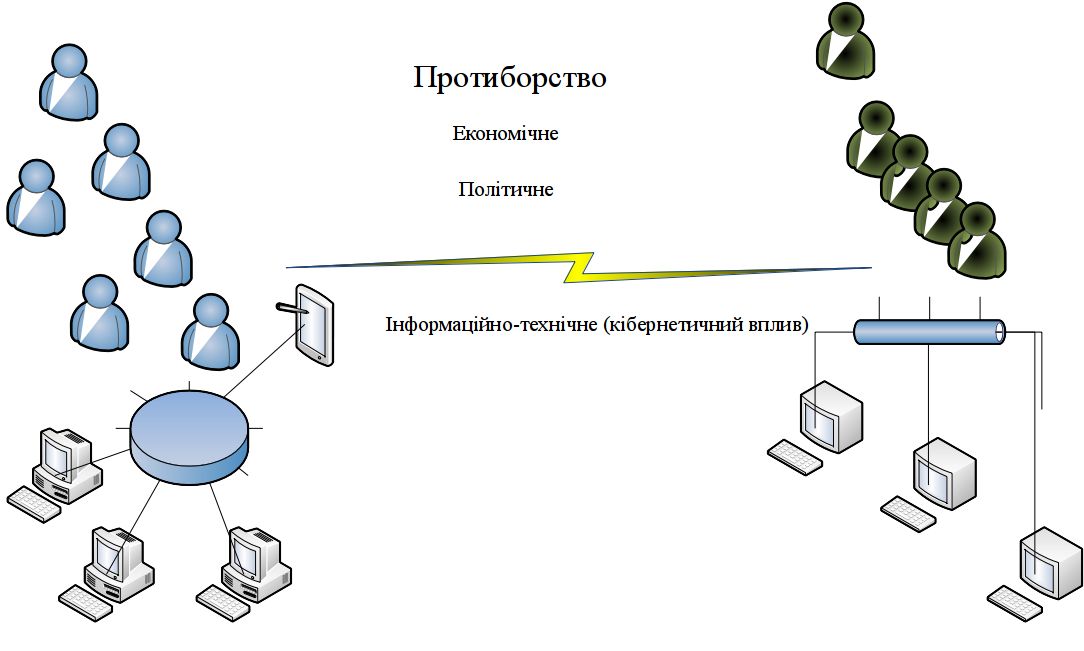
\includegraphics[width=15cm]{pic_cyber1.png}
    \caption{схема кібернетичного впливу}
    \label{fig:cyber_attack}
\end{figure}

Одним із підходів до підготовки військових фахівців, які здатні підтримувати безпеку у кібернетичному просторі – комунікаційному просторі, який охоплює комп’ютерні мережі та електронні пристрої, що використовуються для збереження, обробки та обміну інформацією є підготовка фахівців, що починається з формуванння бази до кваліфікаційного рівня бакалавр, а саме проходження циклів підготовки.
Підготовка фахівців з інформаційної безпеки (Рис \,\ref{fig:cyber_attack})

починається у циклі професійної і практичної підготовки, де на вивчаємих дисциплінах майбутніми фахівцями вивчаються матеріали, для формування загальних знань з комп’ютерних наук, вивчаються мови програмування, технології створення програмних продуктів, архітектура комп’ютерних та операційних  систем. Але щоб стати фахівцем, потрібна додаткова підготовка яка отримується після захисту кваліфікаційної роботи, майбутні фахівці розподіляються за спеціалізаціями підготовки, фахівці формуються відповідно до спеціалізації.

На етапі підготовки згідно спеціалізації вивчаються такі дисципліни як:
\begin{itemize}
\itemЕксплуатація та бойове застосування програмних засобів інформаційної боротьби в комп’ютеризованих системах та мережах спеціального призначення;
\itemМетодологічні основи інформаційної боротьби в комп’ютеризованих системах та мережах спеціального призначення;
\itemТехнології побудови програмних засобів інформаційної боротьби та ін.
\end{itemize}


\begin{figure}[h]
    \centering
    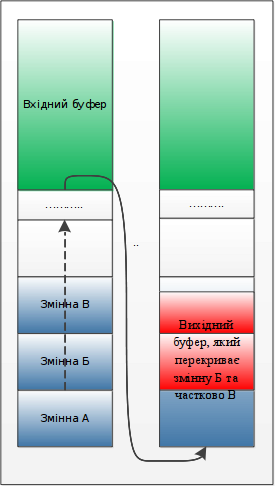
\includegraphics[height=10cm]{pic_bo_0.png}
    \caption{схема переповнення буфера}
    \label{fig:buffer_overflow}
\end{figure}

На етапі підготовки згідно спеціалізації потрібно приділяти багато уваги практичній підготовці та інтерактивному навчанню. Для цьго пропонується підхід до створення тренувального середовища із завідомо впровадженими вразливостями для нав’язування тестових впливів. Це середовище може слугувати матеріалом для вивчення вищеназваних дисциплін, як для відпрацювання технології побудови програмних засобів інформаційної боротьби,  для відпрацювання методології впливу на програмні продукти, а також використання програм для сканування вразливостей.

Необхідно виділити найбільш небезпечні вразливості для створення такої системи, кожна з уразливостей потребує детального вивчення, це окрема спеціалізація,  яка рамках підготовки фахівця з інформаційної безпеки потребує глибокого дослідження.
Досить розповсюдженим видом комп'ютерних атак на інформаційні системи є атака на переповнення буфера.
Переповнення буфера було та залишається дуже важливою проблемою в аспекті безпеки програмного забезпечення. Переповнення буфера (англ. buffer overflow або англ. buffer overrun), це явище, при якому програма, під час запису даних в буфер, перезаписує дані за межами буфера.
(Рис.\,\ref{fig:buffer_overflow})


Це може викликати несподівану поведінку, включно з помилками доступу до даних, невірними результатами, збоєм програми або дірою в системі безпеці.
Переповнення буфера може бути викликане недостатньою перевіркою вхідних даних. Воно є базою для багатьох уразливостей в програмних продуктах і може бути злонамірено використане.

Проблема переповнення буфера з роками тільки ускладнювалася, з'являлися типи атак, в результаті були розроблені принципово нові атаки на переповнення буфера.
Оскільки значна частка програмного забезпечення створюється на мові C/C++, в якій немає вбудованих засобів обробки рядків - а саме контролю розподілу пам’яті, тому вони використовують небезпечний програмний код, що не перевіряє довжину буфера, у який записуються зовнішні дані, отримані ззовні, внаслідок чого можливість перезапису інших даних програми, включаючи код, що дозволяє змінити виконання програми, незалежно коду. Атаки, в основному, здійснюються на програмні застосування, виконуються в привілейованому режимі, що дозволяє підняти рівень привілеїв для виконання шкідливого коду.
Зробивши аналіз найбільш поширених прийомів техніки переповнення буферу можна зробити висновок що фахівцям в даній предметній області необхідно мати глибокі знання в таких дисциплінах як:
\begin{itemize}
\itemопераційні системи(знання архітектури ОС Linux/Unix-like/WinX);
\itemсистемне, мережеве програмування (низькорівневе);
\itemтеорії побудови компіляторів / інтерпретаторів – теорія кінцевих автоматів;
\itemпрактичні навички використання засобів відлагодження та дослідження програмних продуктів;
\end{itemize}

\upshape{Типові ситуації використання переповнення буфера.}

Техніки використання уразливості через переповнення буфера залежать від архітектури, операційної системи і ділянки пам'яті 
%(рис.1.5.)
.
Існують наступні види переповнення буфера:
\begin{itemize}
\itemпереповнення у стекові (stack smashing - зрив стеку), який полягає у перезаписі адреси повернення з вразливої функції, що призводить до виконання коду(існуючого або підготовленого зловмисником) за адресом, вказаним атакуючим;
\itemпереповнення в сегментах даних та динамічних областях (DATA, BSS, HEAP overflow), яке являє собою корекцію набору даних, керуючих алгоритмом програми, а також вказівників на функції, класи та управління. 
\end{itemize}


Технічно освідомлений і злонамірений користувач може використати стекове переповнення буфера так:
\begin{enumerate}
\itemДля перезапису локальної змінної, змінивши тим самим перебіг програми на більш вигідний для нападника.
\itemДля перезапису адреси повернення в стековому кадрі. Коли буде виконане повернення з функції, виконання програми відновиться за адресою, вказаною нападником (зазвичай це адреса буфера поля вводу). Такий спосіб найбільш розповсюджений в архітектурах, де стек росте донизу (наприклад в архітектурі x86).
\itemДля перезаписів вказівника на функцію, або обробника винятків, що будуть виконані згодом. 
\end{enumerate}

Два основних типи даних, які дозволяють здійснити переповнення буфера в цих мовах — рядки і масиви. Таким чином, використання бібліотек для рядків і спискових структур даних, які були розроблені для запобігання і/або виявлення переповнень буфера, дозволить уникнути уразливостей.
Шелкод (Корисне навантаження) ( англ. {\it shellcode}, код запуску оболонки) - це двійковий виконуваний код, який зазвичай передає управління командному процесору,  наприклад `{\it / bin / sh}'  {\it Unix Shell}, {\it command.com} в {\it MS-DOS} і {\it cmd.exe} в операційних системах {\it Microsoft Windows}.  Шелкод може бути використаний як корисне навантаження експлойту, що забезпечує зловмисникові доступ до командного інтерпретатра (англ.{\it shell}) в комп'ютерній системі.

При експлуатації віддаленої уразливості шелкод може відкривати заздалегідь заданий порт {\it TCP} уразливого комп'ютера, через який буде здійснюватися подальший доступ до командної оболонці, такий код називається прив'язує до порту ( англ. {\it port binding shellcode}).  Якщо шелкод здійснює підключення до порту комп'ютера атакуючого, що проводиться з метою обходу брандмауера або {\it NAT}, то такий код називається зворотної оболонкою ( англ. {\it reverse shell shellcode}).
Шелкод зазвичай впроваджується в пам'ять експлуатованої програми, після чого на нього передається управління шляхом переповнення стека, або при переповненні буфера в купі, або використовуючи атаки форматної рядка.  Передача управління шелкоду здійснюється перезаписом адреси повернення в стеку адресою впровадженого шелкоду, перезаписом адрес викликаються функцій або зміною обробників переривань.  Результатом цього є виконання шелкоду, який відкриває командний рядок для використання зломщиком.

Розрізняють два типи шелкоду :
\begin{itemize}
\itemлокальний (впровадження та виконання можливе тільки за безпосереднього доступу зловмисника до КС)
\itemвіддалений (атака з віддаленої машини). 
\end{itemize}

Локальний шелкод використовується зловмисником, коли він обмежений в правах комп’ютерної системи, але може використати вразливість в програмному забезпеченні даної системи з підняттям привілеїв до того рівня що і цільовий процес.

Віддалений шелкод використовується хакерами для захоплення контролю над процесом на віддаленій машині в локальній мережі чи в інтернеті. У разі успішного його виконання, хакер матиме можливість отримати доступ над машиною по мережі. Віддалені шелкоди переважно використовують  {\it TCP/IP}-зєднання для забезпечення атакуючого доступом до командної оболонки. Такий шелкод може бути класифікований по тому, як він встановлює з’єднання.: якщо код може встановити з’єднання, його називають ``{\it reverse shell}'' або “{\it connect-back shellcode}”
%(рис.1.6.)
, так як він з’єднується з машиною атакуючого. З іншого боку, якщо зловмисник потребує встановити з’єднання, то такий шелкод називають “{\it  bindshell}”, так як він відкриває і прослуховує порт, по якому зловмисник може під’єднатися і отримати контроль над системою. Є третій тип, менш використовуваний, має назву “{\it socket-reuse shellcode}”. Цей тип шелкоду іноді використовується, коли експлойт встановлює з’єднання з вразливим процесом, який до його запуску не закрив з’єднання. Тому він може використати з’єднання для комунікації з хакером для віддаленого управління системою. Цей тип шелкоду є складним в реалізації так як він повинен виконати пошук вразливого процесу, який має відкрите з’єднання.

\pagebreak

\section{Дослідження початкового тексту як метод виявлення потенційно-небезпечних дефектів програм.}
\label{1section:id3}
На сьогоднішній час існує низка засобів для аналізу програм як у вигляді вихідних текстів так і у двійковому коді.
Для виявлення вразливостей захисту в програмах застосовують такі інструментальні засоби:
\begin{itemize}
\itemдинамічні відлагоджувачі. Інструменти, які дозволяють виробляти налагодження програми в процесі її виконання;
\itemстатичні аналізатори (статичні відлагоджувачі).
\end{itemize}

Інструменти, які використовують інформацію, накопичену в ході статичного аналізу досліджуваної програми.

Статичні аналізатори вказують на ті місця в програмі, в яких можливо знаходиться помилка. Ці підозрілі фрагменти коду можуть, як містити помилку, так і не нести ніякої небезпеки для виконання програми. Наявність вихідних кодів програми істотно спрощує пошук вразливостей.
Розглянемо декілька інструментів для аналізу вихідних текстів досліджуваних програм:

Інструмент {\it BOON}, який на основі глибокого семантичного аналізу автоматизує процес сканування вихідних текстів на Сі в пошуках уразливих місць, здатних призводити до переповнення буферу. Він виявляє можливі дефекти, припускаючи, що деякі значення є частиною неявного типу з конкретним розміром буфера.

{\it CQual} - інструмент аналізу для виявлення помилок в Сі-програмах. Програма розширює мову Сі додатковими обумовленими користувачем специфікаторами типу. Програміст коментує свою програму з відповідними специфікаторами, і {\it cqual} перевіряє помилки. Неправильні анотації вказують на потенційні помилки. {\it Сqual} може використовуватися, щоб виявити потенційну уразливість форматною рядка.

{\it MOPS} - інструмент для пошуку вразливостей в захисті в програмах на Сі. Його призначення: динамічне коректування, що забезпечує відповідність програми на Сі статичної моделі. {\it MOPS} використовує модель аудиту програмного забезпечення, яка покликана допомогти з'ясувати, чи відповідає програма набору правил, визначеному для створення безпечних програм.

{\it ITS4}. Простий інструмент, який статично переглядає вихідний Сі / Сі++ - код для виявлення потенційних вразливостей захисту. Він зазначає виклики потенційно небезпечних функцій, таких, наприклад, як {\it strcpy / memcpy}, і виконує поверхневий семантичний аналіз, намагаючись оцінити, наскільки небезпечний такий код, а так само дає поради щодо його поліпшення.

{\it RATS}. Утиліта {\it RATS (Rough Auditing Tool for Security)} обробляє код, написаний на Сі / Сі++, а також може обробити ще і скрипти на {\it Perl, PHP і Python. RATS} переглядає вихідний текст, знаходячи потенційно небезпечні звернення до функцій. Мета цього інструменту - не остаточно знайти помилки, а забезпечити обгрунтовані висновки, спираючись на які фахівець зможе вручну виконувати перевірку коду.{\it RATS} використовує поєднання перевірок надійності захисту від семантичних перевірок в {\it ITS4} до глибокого семантичного аналізу в пошуках дефектів, здатних привести до переповнення буфера, отриманих з {\it MOPS}.

{\it Flawfinder}. Як і {\it RATS}, це статичний сканер вихідних текстів програм, написаних на {\it С/С++}. Виконує пошук функцій, які найчастіше використовуються некоректно, присвоює їм коефіцієнти ризику (спираючись на таку інформацію, як передані параметри) і складає список потенційно вразливих місць, впорядковуючи їх за ступенем ризику.

Всі ці інструменти схожі і використовують тільки лексичний і найпростіший синтаксичний аналіз. Тому результати, видані цими програмами, можуть містити до 100\% помилкових повідомлень.

{\it Bunch} - засіб аналізу та візуалізації програм на Сі, яке будує граф залежностей, що допомагає аудитору розібратися в модульній структурі досліджуваної програми.

{\it Frama-C} - відкритий, інтегрований набір інструментів для аналізу вихідного коду на мові Сі. Набір включає {\it ACSL (ANSI / ISO C Specification Language)} - спеціальна мова, що дозволяє детально описувати специфікації функцій Сі, наприклад, вказати діапазон допустимих вхідних значень функції і діапазон нормальних вихідних значень.
\begin{quote}

Цей інструментарій допомагає виробляти такі дії:
\end{quote}
\begin{itemize}
\item {} 
здійснювати формальну перевірку коду;

\item {} 
шукати потенційні помилки виконання;

\item {} 
провести аудит або рецензування коду;

\item {} 
проводити реверс-інжиніринг коду для поліпшення розуміння структури програмного коду;

\item {} 
генерувати формальну документацію.

\end{itemize}

Також при відсутності вихідного тексту для аналізу програмного коду можна використовувати динамічні відлагоджувачі, які також можуть допомогти виявити помилки в коді, які допущені компілятором.
Найпоширенішими відлагоджувачами на даний момент є {\it SoftIce, OllyDebug, IDA Pro, GDB:}

{\it SoftIce} – всім відомий відлагоджувальник для ОС сімейства {\it Windows}, який працює в режимі ядра, що дозволяє відлагоджувати драйвера та різного роду сервіси що працюють в привілейованому режимі процесора. Працює в обхід {\it MS Debugging API}, що дуже ускладнює реалізацію захисту від відлагодження. {\it SoftICE}  був спочатку розроблений компанією {\it NuMega}, яка включала його в пакет програм для швидкої розробки високопродуктивних драйверів під назвою {\it Driver Studio}, який пізніше був придбаний {\it Compuware}.

{\it OllyDebug} – це 32-бітний відлагоджувальник працюючий в непривілейованому режимі процесора. Він має достатньо зручний інтерфейс та корисні функції які значно полегшують процес від лагодження.  В {\it OllyDBG} вбудований спеціальний аналізатор, який розпізнає і візуально позначає процедури, цикли, константи і рядки, звернення до функцій {\it API}, параметри цих функцій і т.п.

{\it IDA Pro} – це одночасно інтерактивний дизасемблер і відлагоджувальник. Він дозволяє отримати асемблерний текс, який може бути застосований для аналізу роботи програми. Варто зазначити, що вбудований відлагоджувальник доволі примітивний, працює через {\it MS Debugging API (в NT)} і через бібліотеку ptrace (в {\it UNIX}), що робить його легкорозпізнаємим для захисних механізмів. Сильною стороною цього продукту є саме дизасемблер, який на сьогодні генерує якісний вихідний текс. Окрім цього існує велика кількість плагінів під даний програмний продукт, що значно розширює його можливості. Також можливе написання плагінів на скрипкових мовах – є підтримка {\it Ruby, Python}.

{\it GDB - GNU Debugger} – основний відлагоджувальник під {\it UNIX}, орієнтований на зовсім інший тип мислення, аніж всі вищеперераховані відлагоджувальники. Це не просто інтерактивний відлагоджувальник – це модуль управління виконанням програм з гнучким і потужним інтерфейсом. Негативною стороною даного відлагоджувальника є відсутність аналізу захисних механізмів програм, тому у разі їх присутності в коді – процес відлагоджування стає неможливим.

Дані програмні засоби добре справляються з заявленими ними завданнями, але враховуючи тенденції теперішніх технологій та стрімкий ріст розмірів як вихідних текстів програм так і їх двійкових образів, завдання швидкого аналізу дещо ускладюється насамперед тим, що результати аналізу містять надмірну кількість інформації, яку такок потрібно аналізувати. Тому виникає потреба в більш загальному аналізі характеристик коду, який дасть якісну оцінку окремих частин досліджуванної програми, що дозволить диференціювати задачу аналізу та правильно його організувати.

Завдання оцінки інтегрованих властивостей програм в певній мірі вирішують так звані метрики коду. 

Метрика якості програм - система вимірювань якості програм . Ці виміри можуть проводитися на рівні критеріїв якості програм або на рівні окремих характеристик якості. У першому випадку система вимірювань дозволяє безпосередньо порівнювати програми за якістю. При цьому самі виміри не можуть бути проведені без суб'єктивних оцінок властивостей програм. У другому випадку вимірювання характеристик можна виконати об'єктивно і достовірно, але оцінка якості ПЗ в цілому буде пов'язана з суб'єктивною інтерпретацією одержуваних оцінок.

\pagebreak

\section*{Висновки}
\addcontentsline{toc}{section}{Висновки}
Отже, в зрізі теперішніх тенденцій інформаційних технологій  - а саме стрімкого росту розмірів як вихідних текстів програм так і їх двійкових образів виникає потреба в більш загальному аналізі характеристик коду, який дасть якісну оцінку окремих частин досліджуванної програми, що дозволить диференціювати задачу аналізу та правильно його організувати.


\chapter{ТЕОРЕТИЧНІ ЗАСАДИ ПІДВИЩЕННЯ ЕФЕКТИВНОСТІ ПОШУКУ (ДОСЛІДЖЕННЯ) ПОТЕНЦІЙНО-НЕБЕЗПЕЧНИХ ДЕФЕКТІВ ПРОЕКТУВАННЯ ТА РЕАЛІЗАЦІЇ ЦІЛЬОВИХ ПРОГРАМ}
\label{2section::doc}\label{2section:id1}

%TODO зкоротити опис метрик


\section{Інтегровані властивості цільової програми}
\label{2section:id2}
На відміну від більшості галузей матеріального виробництва, в питаннях проектів створення ПЗ неприпустимі прості підходи, засновані на множенні трудомісткості на середню продуктивність праці. Це викликано, насамперед, тим, що економічні показники проекту нелінійно залежать від обсягу робіт, а при обчисленні трудомісткості допускається велика похибка.

Тому для вирішення цього завдання використовуються комплексні і досить складні методики, які вимагають високої відповідальності в застосуванні і певного часу на адаптацію (настройку коефіцієнтів).

Сучасні комплексні системи оцінки характеристик проектів створення ПЗ можуть бути використані для вирішення наступних завдань:
\begin{itemize}
\item {} 
попередня, постійна і підсумкова оцінка економічних параметрів проекту: трудомісткість, тривалість, вартість;

\item {} 
оцінка ризиків по проекту: ризик порушення строків та невиконання проекту, ризик збільшення трудомісткості на етапах налагодження та супроводження проекту та пр;

\item {} 
прийняття оперативних управлінських рішень - на основі відстеження певних метрик проекту можна своєчасно попередити виникнення небажаних ситуацій і усунути наслідки непродуманих проектних рішень.

\end{itemize}

Для вимірювання характеристик і критеріїв якості використовують метрики.

Метрика якості програм - система вимірювань якості програм . Ці виміри можуть проводитися на рівні критеріїв якості програм або на рівні окремих характеристик якості. У першому випадку система вимірювань дозволяє безпосередньо порівнювати програми за якістю. При цьому самі виміри не можуть бути проведені без суб'єктивних оцінок властивостей програм. У другому випадку вимірювання характеристик можна виконати об'єктивно і достовірно, але оцінка якості ПЗ в цілому буде пов'язана з суб'єктивною інтерпретацією одержуваних оцінок.

У дослідженні метрик ПО розрізняють два основних напрямки:
\begin{quote}
\begin{itemize}
\item {} 
Пошук метрик, що характеризують найбільш специфічні властивості програм, тобто метрик оцінки самого ПЗ;

\item {} 
Використання метрик для оцінки технічних характеристик і факторів розробки програм, тобто метрик оцінки умов розробки програм.

\end{itemize}

По виду інформації, одержуваної при оцінці якості ПО метрики можна розбити на три групи:
\begin{itemize}
\item {} 
Метрики, що оцінюють відхилення від норми характеристик вихідних проектних матеріалів . Вони встановлюють повноту заданих технічних характеристик вихідного коду.

\item {} 
Метрики, що дозволяють прогнозувати якість розроблюваного ПЗ. Вони задані на безлічі можливих варіантів рішень поставленого завдання і їх реалізації і визначають якість ПЗ, яке буде досягнуто в результаті.

\item {} 
Метрики, за якими приймається рішення про відповідність кінцевого ПО заданим вимогам . Вони дозволяють оцінити відповідність розробки заданим вимогам .

\end{itemize}
\end{quote}


\subsection{Основні намрямки застосуваня метрик}
\label{2section:id4}
В даний час у світовій практиці використовується кілька сотень метрик програм. Існуючі якісні оцінки програм можна згрупувати по шести напрямках :
\begin{itemize}
\item {} 
Оцінки топологічної та інформаційної складності програм;

\item {} 
Оцінки надійності програмних систем, що дозволяють прогнозувати отказовие ситуації ;

\item {} 
Оцінки продуктивності ПО і підвищення його ефективності шляхом виявлення помилок проектування ;

\item {} 
Оцінки рівня мовних засобів і їх застосування;

\item {} 
Оцінки труднощі сприйняття і розуміння програмних текстів, орієнтовані на психологічні фактори, суттєві для супроводу і модифікації програм;

\item {} 
Оцінки продуктивності праці програмістів для прогнозування термінів розробки програм і планування робіт зі створення програмних комплексів.

\end{itemize}


\subsection{Метричні шкали}
\label{2section:id5}
Залежно від характеристик і особливостей застосовуваних метрик їм ставляться у відповідність різні вимірювальні шкали.

Номінальною шкалою відповідають метрики, що класифікують програми на типи за ознакою наявності або відсутності деякої характеристики без урахування градацій.

Порядкової шкалою відповідають метрики, що дозволяють ранжувати деякий характеристики шляхом порівняння з опорними значеннями, тобто вимір за цією шкалою фактично визначає взаємне положення конкретних програм.

Інтервального шкалою відповідають метрики, які показують не тільки відносне положення програм, але і те, як далеко вони відстоять один від одного.

Відносній шкалі відповідають метрики, що дозволяють не тільки розташувати програми певним чином і оцінити їх положення відносно один одного, а й визначити, як далеко оцінки відстоять від кордону, починаючи з якої характеристика може бути виміряна.

Метрика складності:
При оцінці складності програм, як правило, виділяють три основні групи метрик:
\begin{itemize}
\item {} 
Метрики розміру програм

\item {} 
Метрики складності потоку управління програм

\item {} 
Метрики складності потоку даних програм

\end{itemize}

Метрика розміру програм.

Оцінки першої групи найбільш прості і, очевидно, тому отримали широке поширення. Традиційною характеристикою розміру програм є кількість рядків вихідного тексту. Під рядком розуміється будь-який оператор програми, оскільки саме оператор, а не окремо взята рядок є тим інтелектуальним '' квантом '' програми, спираючись на який можна будувати метрики складності її створення.
Безпосереднє вимірювання розміру програми, незважаючи на свою простоту, дає хороші результати. Звичайно, оцінка розміру програми недостатня для прийняття рішення про її складності, але цілком застосовна для класифікації програм, істотно різняться обсягами. При зменшенні відмінностей в обсязі програм на перший план висуваються оцінки інших факторів, що впливають на складність . Таким чином, оцінка розміру програми є оцінка за номінальною шкалою, на основі якої визначаються тільки категорії програм без уточнення оцінки для кожної категорії .

До групи оцінок розміру програм можна віднести також і метрику Холстеда .

Метрика Холстеда.
Основу метрики Холстеда складають чотири вимірюваних характеристики програми :
n1 - число унікальних операторів програми, включаючи символи -
роздільники, імена процедур і знаки операцій ( словник операторів ) ;
n2 - число унікальних операндів програми ( словник операндів ) ;
N1 - загальне число операторів в програмі ;
N2 - загальне число операндів в програмі.
Спираючись на ці характеристики, одержувані безпосередньо при аналізі вихідних текстів програм, М. Холстед вводить такі оцінки:
словник програми
 n1 = n1 + n2,
довжину програми
 N = N1 + N2, ( 1 )
обсяг програми
 V = N * log2 ( n ) ( біт).

Метрика складності потоку управління програми.
Друга найбільш представницька група оцінок складності програм - метрики складності потоку керування програм. Як правило, за допомогою цих оцінок оперують або щільністю керуючих переходів усередині програм, або взаємозв'язками цих переходів .

І в тому і в іншому випадку стало традиційним уявлення програм у вигляді керуючого орієнтованого графа G = (V, E), де V - вершини, відповідні операторам, а E - дуги, відповідні переходам .

Метрика Маккейба.
Вперше графічне представлення програм було запропоновано МакКейб . Основний метрикою складності він пропонує вважати цикломатическая складність графа програми, або, як її ще називають, цикломатичне число МакКейб, що характеризує трудомісткість тестування програми .
Для обчислення цикломатическая числа МакКейб Z (G ) застосовується формула
Z( G) = e - v +2 p,
де e - число дуг орієнтованого графа G ;
v - число вершин ;
p - число компонентів зв'язності графа.
Число компонентів зв'язності графа можна розглядати як кількість дуг, які необхідно додати для перетворення графа в сильно зв'язний . Сильний зв'язковим називається граф, будь-які дві вершини якого взаємно досяжні. Для графів коректних програм, тобто графів, що не мають недосяжних від точки входу ділянок і ''висячих'' точок входу і виходу, сильно зв'язний граф, як правило, виходить шляхом замикання дугою вершини, що позначає кінець програми, на вершину, що позначає точку входу в цю програму.
По суті Z (G ) визначає число лінійно незалежних контурів у Сильно зв'язкового графі . Інакше кажучи, цикломатичне число МакКейб показує необхідну кількість проходів для покриття всіх контурів сильно зв'язного графа або кількість тестових прогонів програми, необхідних для вичерпного тестування за критерієм '' працює кожна гілка'' .
Для зображеної програми, цикломатичне число при e = 10, v = 8, p = 1 визначиться як Z ( G) = 10-8 +2 = 4 .

Цикломатичне число залежить тільки від кількості предикатів, складність яких при цьому не враховується. 
Обидва оператора припускають єдине розгалуження і можуть бути представлені одним і тим же графом. Очевидно, цикломатичне число буде для обох операторів однаковим, що не відображає складності предикатів, що досить істотно при оцінці програм.

Метрика Маєрса.
Виходячи з цього Г. Майерс запропонував розширення цієї метрики . Суть підходу Г. Майерса полягає в представленні метрики складності програм у вигляді інтервалу {[}Z (G), Z ( G) + h {]} . Для простого предиката h = 0, а для n-місних предикатів h = n - 1 . Таким чином, перший оператору відповідає інтервал {[} 2,2 {]}, а другий - {[} 2,6 {]} .
По ідеї така метрика дозволяє розрізняти програми, представлені однаковими графами. На жаль, інформація про результати використання цього методу відсутня, тому нічого не можна сказати про його застосовності .

Метрика підрахунку точок перетину.
Розглянемо метрику складності програм, що отримала назву '' підрахунок точок перетину '', авторами якої є М.Вудвард, М.Хенель і Д.Хідлі. Метрика орієнтована на аналіз програм, при створенні яких використовувалося неструктурні кодування на таких мовах, як мова асемблера і фортран.
У графі програми, де кожному оператору відповідає вершина, тобто не виключені лінійні ділянки, при передачі управління від вершини a до b номер оператора a дорівнює min ( a, b ), а номер оператора b - max ( a, b ) . Точка перетину дуг з'являється, якщо
min ( a, b ) \textless{} min ( p, q ) \textless{} max ( a, b ) \& max ( p, q ) \textgreater{} max ( a, b ) \textbar{}
min ( a, b ) \textless{} max ( p, q ) \textless{} max ( a, b ) \& min ( p, q ) \textless{} min ( a, b ) .
Іншими словами, точка перетину дуг виникає у разі виходу управління за межі пари вершин ( a, b ) (рис. 3 ) .
Кількість точок перетину дуг графа програми дає характеристики не структурованості програми .

Метрика Джилба.
Однією з найбільш простих, але, як показує практика, досить ефективних оцінок складності програм є метрика Т. Джилба, в якій логічна складність програми визначається як насиченість програми виразами типу IF- THEN - ELSE . При цьому вводяться дві характеристики : CL - абсолютна складність програми, що характеризується кількістю операторів умови; cl - відносна складність програми, що характеризується насиченістю програми операторами умови, тобто cl визначається як відношення CL до загального числа операторів.
Використовуючи метрику Джилба, ми доповнили її ще однією складовою, а саме характеристикою максимального рівня вкладеності оператора CLI, що дозволило не тільки уточнити аналіз по операторам типу IF- THEN - ELSE, але й успішно застосувати метрику Джилба до аналізу циклічних конструкцій.

Метрика граничних значень.
Великий інтерес представляє оцінка складності програм за методом граничних значень .
Введемо кілька додаткових понять, пов'язаних з графом програми.
Нехай G = (V, E) - орієнтований граф програми з єдиною початковою і єдиною кінцевою вершинами. У цьому графі число входять вершин у дуг називається негативною ступенем вершини, а число що виходять з вершини дуг - позитивної ступенем вершини . Тоді набір вершин графа можна розбити на дві групи: вершини, у яких позитивна ступінь \textless{}= 1 ; вершини, у яких позитивна ступінь \textgreater{} = 2 .
Вершини першої групи назвемо приймаючими вершинами, а вершини другої групи - вершинами відбору.
Для отримання оцінки за методом граничних значень необхідно розбити граф G на максимальне число подграфов G `, що задовольняють таким умовам: вхід в подграф здійснюється тільки через вершину відбору; кожен подграф включає вершину ( звану надалі нижньою межею подграфа ), в яку можна потрапити з будь іншої вершини подграфа . Наприклад, вершина відбору, поєднана сама з собою дугою - петлею, утворює подграф.
Число вершин, що утворюють такий подграф, одно скоригованої складності вершини відбору. Кожна приймаюча вершина має скориговану складність, рівну 1, крім кінцевої вершини, скоригована складність якої дорівнює 0 . Скориговані складності всіх вершин графа G підсумовуються, утворюючи абсолютну граничну складність програми . Після цього визначається відносна гранична складність програми :

S0 = 1 - ( v - 1 ) / Sa,
де S0 - відносна гранична складність програми ; Sa - абсолютна гранична складність програми ; v - загальне число вершин графа програми .

Метрика складності потоку даних.
Інша група метрик складності програм - метрики складності потоку даних, тобто використання, конфігурації і розміщення даних в програмах.

Метрика обігу до глобальних змінних.
Розглянемо метрику, що зв'язує складність програм із зверненнями до глобальних змінних .
Пара '' модуль - глобальна змінна'' позначається як ( p, r ), де p - модуль, що має доступ до глобальної змінної r . Залежно від наявності в програмі реального обігу до змінної r формуються два типи пар '' модуль - глобальна змінна'' : фактичні і можливі . Можливе звернення до r за допомогою p показує, що область існування r включає в себе p.

Характеристика Aup говорить про те, скільки разів модулі Up дійсно отримували доступ до глобальних змінних, а число Pup - скільки разів вони могли б отримати доступ.

Відношення числа фактичних звернень до можливих визначається

\begin{equation}
 Rup = Aup / Pup
\end{equation}

Ця формула показує наближену ймовірність посилання довільного модуля на довільну глобальну змінну. Очевидно, чим вище ця вірогідність, тим вище ймовірність несанкціонованої зміни якої-небудь змінної, що може істотно ускладнити роботи, пов\dq язані з модифікацією програми. На жаль, поки не можна сказати, наскільки зручний і точний цей метод на практиці, так як немає відповідних статистичних даних.

Метрика Спен.
Визначення Спен грунтується на локалізації звернень до даних всередині кожної програмної секції. Спен - це число тверджень, які містять даний ідентифікатор, між його першим і останнім появою в тексті програми . Отже, ідентифікатор, що з'явився n раз, має Спен, рівний n - 1 . При великому Спен ускладнюється тестування і налагодження.

Метрика Чепіна.
Суть методу полягає в оцінці інформаційної міцності окремо взятого програмного модуля за допомогою аналізу характеру використання змінних зі списку вводу-виводу.
Всі безліч змінних, складових список введення-виведення, розбивається на 4 функціональні групи:

\begin{itemize}
\item P - що вводяться змінні для розрахунків та для забезпечення виведення.
Прикладом може служити використовувана в програмах лексичного аналізатора змінна, що містить рядок вихідного тексту програми, тобто сама змінна не модифікується, а лише містить вихідну інформацію .

\item M - модифікуються, або створювані всередині програми змінні.

\item C - змінні, що беруть участь в управлінні роботою програмного модуля (керуючі змінні).

\item T - які не використовуються в програмі ( '' паразитні '' ) змінні. Оскільки кожна змінна може виконувати одночасно кілька функцій, необхідно враховувати її в кожній відповідній функціональній групі . 
\end{itemize}

Далі вводиться значення метрики Чепіна :

Q = a1 * P + a2 * M + a3 * C + a4 * T, ( 4 )
де a1, a2, a3, a4 - вагові коефіцієнти .

Вагові коефіцієнти у виразі ( 4 ) використані для відбиття різного впливу на складність програми кожної функціональної групи . На думку автора метрики, найбільшу вагу, що дорівнює трьом, має функціональна група C, так як вона впливає на потік управління програми . Вагові коефіцієнти решти груп розподіляються наступним чином : a1 = 1, a2 = 2, a4 = 0.5 . Ваговий коефіцієнт групи T НЕ дорівнює 0, оскільки '' паразитні '' змінні не збільшують складність потоку даних програми, але іноді ускладнюють її розуміння . З урахуванням вагових коефіцієнтів вираз ( 4 ) приймає вигляд:

Q = P + 2M + 3C + 0.5T
Слід зазначити, що розглянуті метрики складності програм засновані на аналізі вихідних текстів програм і графів, що забезпечує єдиний підхід до автоматизації з розрахунку .


Метрика стилістики та зрозумілої програми

Метрика рівня коментування програм.
Найбільш простий метрикою стилістики та зрозумілості програм є оцінка рівня коментування програми F :
F = Nком / Nстр, 
де Nком - кількість коментарів у програмі ; Nстр - кількість рядків або операторів вихідного тексту .

Таким чином, метрика F відображає насиченість програми коментарями.

Виходячи з практичного досвіду прийнято вважати, що F = 0.1, тобто на кожні десять рядків програми має припадати мінімум один коментар. Як показують дослідження, коментарі розподіляються по тексту програми нерівномірно: на початку програми їх надлишок, а в середині або в кінці - недолік. Це пояснюється тим, що на початку програми, як правило, розташовані оператори опису ідентифікаторів, що вимагають більш щільного коментування. Крім того, на початку програми також розташовані шапки, що містять загальні відомості про виконавця, характері, функціональне призначення програми і т. п. Така насиченість компенсує недолік коментарів у тілі програми, і тому формула (5) недостатньо точно відображає коментування функціональної частини тексту програми.
Більш вдалий варіант, коли вся програма розбивається на n рівних сегментів і для кожного з них визначається Fi:

Fi = sign ( Nком / Nстр - 0.1),
при цьому

n
F = Сума ( Fi ) .
i = 1
Рівень коментування програми вважається нормальним, якщо виконується умова: F = n . В іншому випадку небудь фрагмент програми доповнюється коментарями до номінального рівня .

Моделі та метрики оцінки якості ПЗ.

Сучасна програмна індустрія за півстоліття шукань накопичила значну колекцію моделей і метрик, що оцінюють окремі виробничі та експлуатаційні властивості ПЗ. Однак гонитва за їх універсальністю, неврахування області застосування розроблюваного ПЗ, ігнорування етапів життєвого циклу програмного забезпечення і, нарешті, необгрунтоване їх використання в різнопланових процедурах прийняття виробничих рішень, істотно підірвало до них довіру розробників і користувачів ПЗ.
Проте, аналіз технологічного досвіду лідерів виробництва ПО показує, наскільки дорого обходиться недосконалість ненаукового прогнозу разрешимости і трудовитрат, складності програм, негнучкість контролю та управління їх розробкою та багато іншого, що вказує на відсутність наскрізної методичної підтримки і призводить зрештою до його невідповідності вимогам користувача, необхідному стандарту і до подальшої болючою і трудомісткою його переробці. Ці обставини, вимагають ретельного відбору методик, моделей, методів оцінки якості ПЗ, врахування обмежень їх придатності для різних життєвих циклах і в межах життєвого циклу, встановлення порядку їх спільного використання, застосування надмірної разномодельного дослідження одних і тих же показників для підвищення достовірності поточних оцінок, накопичення та інтеграції різнорідної метричної інформації для прийняття своєчасних виробничих рішень і заключної сертифікації продукції .

Коротко розглянемо метрики складності. Однією з основних цілей науково -технічної підтримки є зменшення складності ПЗ. Саме це дозволяє знизити трудомісткість проектування, розробки, випробувань і супроводу, забезпечити простоту і надійність виробленого ПЗ. Цілеспрямоване зниження складності ПЗ являє собою багатокрокового процедуру і вимагає попереднього дослідження існуючих показників складності, проведення їх класифікації та співвіднесення з типами програм та їх місцем розташування в життєвому циклі.

Теорія складності програм орієнтована на управління якістю ПЗ і контроль її еталонної складності в період експлуатації. В даний час різноманіття показників (у тій чи іншій мірі описують складність програм) настільки велике, що для їх вживання потрібно попереднє упорядкування . У ряді випадків задовольняються трьома категоріями метрик складності. Перша категорія визначається як словникова метрика, заснована на метричних співвідношеннях Холстеда, цикломатическая заходи Мак- Кейба і вимірах Тейер . Друга категорія орієнтована на метрики зв'язків, що відображають складність відносин між компонентами системи - це метрики Уіна і Вінчестера. Третя категорія включає семантичні метрики, пов'язані з архітектурним побудовою програм та їх оформленням .

Відповідно до іншої класифікації, показники складності діляться на дві групи: складність проектування і складність функціонування . Складність проектування, яка визначається розмірами програми, кількістю оброблюваних змінних, трудомісткістю і тривалістю розробки та ін факторами, аналізується на основі трьох базових компонентів : складність структури програми, складність перетворень ( алгоритмів), складність даних. У другу групу показників віднесені тимчасова, програмна й інформаційна складності, що характеризують експлуатаційні якості ПЗ.

Існує ще ряд підходів до класифікації заходів складності, проте вони, фіксуючи приватні сторони досліджуваних програм, не дозволяють (нехай з великим допущенням ) відобразити загальне, то, чиї виміри можуть лягти в основу виробничих рішень .

Загальним, инвариантно властивим будь-якому ПО (і пов'язаної з його коректністю ), є його СТРУКТУРА . Важливо пов'язати це обставина з певним значенням структурної складності в сукупності заходів складності ПЗ. І більше того, при аналізі структурної складності доцільно обмежитися тільки її топологічними заходами, тобто заходами, в основі яких лежать топологічні характеристики граф - моделі програми . Ці заходи задовольняють переважній більшості вимог, що пред'являються до показників : спільність застосовності, адекватність розглянутого властивості, істотність оцінки, спроможність, кількісне вираження, відтворюваність вимірювань, мала трудомісткість обчислень, можливість автоматизації оцінювання .

Саме топологічні міри складності найчастіше застосовуються у фазі досліджень, формує рішення з управління виробництвом ( в процесах проектування, розробки і випробувань ) і становлять доступний і чутливий еталон готової продукції, контроль якого необхідно регулярно здійснювати в період її експлуатації.

Першою топологічної мірою складності є цикломатическая міра Мак- Кейба . В її основі лежить ідея оцінки складності ПЗ за кількістю базисних шляхів в її керуючому графі, тобто таких шляхів, компонуючи які можна отримати всілякі шляхи з входу графа в виходи . Цикломатичне число l (G) орграфа G з n - вершинами, m - дугами і p - компонентами зв'язності є величина l (G ) = m - n + p .

Має місце теорема про те, що число базисних шляхів в орграфе одно його цикломатическая числу, збільшеному на одиницю . При цьому, цикломатическая складністю ПО Р з керуючим графом G називається величина n (G ) = l (G) +1 = m - n + 2 . Практично цикломатическая складність ПО дорівнює числу предикатів плюс одиниця, що дозволяє обчислювати її без побудови керуючого графа простим підрахунком предикатів . Дана міра відображає психологічну складність ПЗ.

До достоїнств заходи відносять простоту її обчислення і повторюваність результату, а також наочність і змістовність інтерпретації. Як недоліки можна відзначити: нечутливість до розміру ПО, нечутливість до зміни структури ПО, відсутність кореляції зі структурованістю ПО, відсутність відмінності між конструкціями Розвилка і Цикл, відсутність чутливості до вкладеності циклів . Недоліки цикломатическая заходи призвело до появи її модифікацій, а також принципово інших заходів складності.

Дж. Майерс запропонував як міри складності інтервал {[} n 1 ¸ n 2 {]}, де n 1 - цикломатическая міра, а n 2 - число окремих умов плюс одиниця . При цьому, оператор DO вважається за одну умову, а CASE cn - исходами за n - 1 - умов. Введена міра отримала назву інтервального заходом.

У. Хансену належить ідея брати в якості міри складності ПО пару \{ цикломатическая число, число операторів \} . Відома топологічна міра Z ( G), чутлива до структурованості ПЗ. При цьому, вона Z ( G) = V (G) ( дорівнює цикломатическая складності ) для структурованих програм і Z ( G) \textgreater{} V (G) для неструктурованих . До варіантів цикломатическая міри складності відносять також міру М (G ) = (V (G), C, Q), де С - кількість умов, необхідних для покриття керуючого графа мінімальним числом маршрутів, а Q - ступінь зв'язності структури графа програми та її протяжність .

До заходів складності, враховує вкладеність керуючих конструкцій, відносять тестуючу міру М і міру Харрісона - Мейджела, що враховують рівень вкладеності і протяжності ПО, міру Пивоварського - цикломатическая складність і глибину вкладеності, і міру Мак- Клур - складність схеми розбиття ПО на модулі з урахуванням вкладеності модулів і їх внутрішньої складності .

Функціональна міра складності Харрісона - Мейджела передбачає приписування кожній вершині графа своєї власної складності (первинної ) і розбиття графа на сфери впливу предикатних вершин. Складність сфери називають наведеною і складають її з первинних складнощів вершин, що входять в сферу її впливу, плюс первинну складність самої предикатной вершини . Первинні складності обчислюються всіма можливими способами. Звідси функціональна міра складності ПО є сума наведених складнощів всіх вершин керуючого графа.

Міра Пивоварського ставить метою врахувати в оцінці складності ПО відмінності не тільки між послідовними і вкладеними керуючими конструкціями, а й між структурованими і неструктурованими програмами. Вона виражається відношенням N ( G) = n * (G) + S Pi, де n * (G) - модифікована цикломатическая складність, обчислена так само, як і V (G), але з однією відмінністю : оператор CASE з n - виходами розглядається як один логічний оператор, а не як n - 1 операторів. Рi - глибина вкладеності i - тієї предикатной вершини .

Для підрахунку глибини укладення предикатних вершин використовується число сфер впливу. Під глибиною вкладеності розуміється число всіх сфер впливу предикатів, які або повністю утримуватися в сфері розглянутої вершини, або перетинаються з нею. Глибина вкладеності збільшується за рахунок вкладеності не самих предикатів, а сфер впливу. Порівняльний аналіз цикломатическая і функціональних заходів з обговорюваної для десятка різних керуючих графів програми показує, що при нечутливості інших заходів цього класу, міра Пивоварського зростає при переході від послідовних програм до вкладених і далі до неструктурованих .

Міра Мак- Клур призначена для управління складністю структурованих програм у процесі проектування. Вона застосовується до ієрархічним схемами розбивки програм на модулі, що дозволяє вибрати схему розбиття з меншою складністю задовго до написання програми . Метрикою виступає залежність складності програми від числа можливих шляхів виконання, числа керуючих конструкцій і числа змінних ( від яких залежить вибір шляху ) . Методика розрахунку складності по Мак-Клур чітко орієнтована на добре структуровані програми.

Тестуючої мірою М називається міра складності, яка задовольняє таким умовам
\begin{enumerate}
\item {} 
Міра складності простого оператора дорівнює 1 ;

\item {} 
М ( \{ F1 ; F2 ;  ; Fn \} ) = Еin M ( Fi);

\item {} 
М ( IF P THEN F1 ELSE F2 ) = 2 MAX ( M ( F1), M (F2 )) ;

\item {} 
М ( WHILE P DO F ) = 2 M ( F).

\end{enumerate}

Міра зростає з глибиною вкладеності і враховує протяжність програми . До тестирующей міру близько примикає міра на основі регулярних вкладень . Ідея цієї міри складності програм полягає в підрахунку сумарного числа символів ( операндів, операторів, дужок ) в регулярному виразі з мінімально необхідним числом дужок, що описує керуючий граф програми . Всі заходи цієї групи чутливі до вкладеності керуючих конструкцій і до протяжності програми . Однак зростає рівень трудомісткості обчислень.

Розглянемо заходи складності, що враховують характер розгалужень . В основі вузловий заходи Вудворда, Хедлі лежить ідея підрахунку топологічних характеристик потоку управління . При цьому, під вузловий складністю розуміється число вузлів передач управління . Дана міра відстежує складність лінеаризації програми і чутлива до структуризації (складність зменшується). Вона застосовна для порівняння еквівалентних програм, переважніше заходи Холстеда, але по спільності поступається міру Мак- Кейба .

Топологічна міра Чена висловлює складність програми числа перетинів кордонів між областями, утвореними блок - схемою програми . Цей підхід застосовується лише до структурованим програмами, що допускає лише послідовне з'єднання керуючих конструкцій . Для неструктурованих програм міра Чена істотно залежить від умовних і безумовних переходів . У цьому випадку можна вказати верхню і нижню межі міри. Верхня - є m +1, де m - число логічних операторів при їх гніздовий вкладеності . Нижня - дорівнює 2 . Коли керуючий граф програми має тільки одну компоненту зв'язності, міра Чена збігається з цикломатическая мірою Мак- Кейба .

Метрики Джілба оцінюють складність графооріентірованних модулів програм відношенням числа переходів за умовою до загального числа виконуваних операторів . Добре зарекомендувала себе метрика, що відноситься число міжмодульних зв'язків до загального числа модулів. Названі метрики використовувалися для оцінки складності еквівалентних схем програм, особливо схем Янова .

Використовуються також міри складності, що враховують історію обчислень, характер взаємодії модулів і комплексні заходи .

Сукупність цикломатическая заходів придатна для оцінювання складності первинних формалізованих специфікацій, які задають в сукупності вихідні дані, цілі та умови побудови шуканого ПЗ. Оцінка цієї первинної програми або порівняння декількох альтернативних її варіантів дозволить спочатку гармонізувати процес розробки ПЗ та від стартової точки контролювати і управляти його поточної результуючої складністю.

Оскільки обробка даних зачіпає наше життя все більшою мірою, помилки ЕОМ можуть тепер мати такі наслідки, як нанесення матеріального збитку, порушення секретності і багато інших, включаючи смерть.

Висока вартість програмного забезпечення - багато в чому наслідок низької надійності. При збільшенні продуктивності програміста ( якщо вимірювати її тільки швидкістю розробки та кодування програми) вартість істотно не зменшується. Спроби збільшити продуктивність програміста можуть у деяких випадках навіть підвищити вартість . Найкращий шлях скорочення вартості - у зменшенні вартості його тестування і супроводу. А це може ( Під супроводом розуміється будь-яке продовження роботи з програмним продуктом, такі як зміни, доповнення тощо з метою забезпечення його подальшої працездатності та відповідності його вимогам часу ) . А це може бути досягнуто не за рахунок інструментів, покликаних збільшити швидкість програмування, а лише в результаті розробки засобів, що підвищують коректність і чіткість при створенні програмного забезпечення.
Основні принципи проектування.

\pagebreak

\section{Застосування метрик інтегрованих властивостей у ході дослідження потенційно-небезпечних дефектів цільових програм}
\label{2section:id8}
В еру стрімкого розвитку ІТ, ефективність кібернетичного впливу залежить не тільки від можливості знайти вразливість, але й від часових характеристик, адже вразливість, яка сьогодні знайдена, завтра може бути вже усунутою. Для забезпечення кращих часових показників необхідно провести правильний розподіл робочих ресурсів для аналізу та розробки засобів впливу - і в ручну таке завдання зайняло б недопустиму кількість часу. Тому використання метрк коду в цьому випадку може допомогти у виборі тих участків, областей коду, де ймовірність успішного впровадження більша.

Тому з однієї сторони код потрібно аналізувати на предмет наявності потенційно-небезпечних дефектів коду, а з іншої - вираховувати його метрики та спрямовувати зусилля в тому напрямку, в якому для цього сприяють і самі властивості, характеристики вихідного тексту.

Як відомо дефект переповнення буферу не завжди може бути використаним для використання в цілях кібернетичного впливу.
Але можна припустити, що в слабо структурованому коді, який містить запутану логіку, велику кількість переходів, розгалужень та змінних набагато легше допустити критичну помилку, яка надасть можливість провести кібернетичний вплив від зацікавленої сторони.

Тому пропоную аналізувати код за допомогою наступних метрик: \begin{itemize}
\item {} 
метрики Холстеда (розмірність коду, словника)

\item {} 
метрики Маккейба (цикломатична складність)

\item {} 
метрики Джилба (складність розгалуження коду)

\end{itemize}

\subsection{Метрика Холстеда}
\label{2section:id10}
До групи оцінок розміру програм можна віднести також метрику Холстеда . За базу прийнятий підрахунок кількості операторів і операндів використовуються у програмі, тобто визначення розміру програми .

Основу метрики Холстеда складають чотири вимірювані характеристики програми : h1 - число унікальних операторів програми, включаючи символи - роздільники, імена процедур і знаки операцій ( словник операторів ) ; h2 - число унікальних операндів програми ( словник операндів ) ; N1 - загальне число операторів в програмі N2 - загальне число операндів в програмі.

Спираючись на ці характеристики, одержувані безпосередньо при аналізі вихідних текстів програм, Холстед вводить такі оцінки

Словник програми h = h1 + h2

Довжину програми N = N1 + N2

Обсяг програми V = N log2 h

Сенс оцінок h і N досить очевидний, тому докладно розглянемо тільки характеристику V.

Кількість символів, що використовуються при реалізації деякого алгоритму, визначається в числі інших параметрів і словників програми h, що представляє собою мінімально необхідне число символів, що забезпечують реалізацію алгоритму .

Далі Холстед вводить h * - теоретичний словник програми, тобто словниковий запас, необхідний для написання програми з урахуванням того, що необхідна функція вже реалізована в даній мові і, отже, програма зводиться до виклику цієї функції. Наприклад, згідно Холстеду можливе здійснення процедури виділення простого числа могло б виглядати так :

CALL SIMPLE ( X, Y ),

де Y- масив чисельних значень, що містять шукане число X.

Теоретичний словник в цьому випадку буде складатися з

n1 * : \{ CALL, SIMPLE (...) \} n1 * = 2 ;

n2 * : \{ X, Y \}, h2 * = 2 ;

h * = h1 * + h2 * дорівнюватиме 4 .

Використовуючи h *, Холстед вводить оцінку V * : V * = h * log2h *,

за допомогою якої описується потенційний обсяг програми, соотвествующий максимально компактно реалізує даний алгоритм.


\subsection{Метрика Маккейба}
\label{2section:id11}
Друга найбільш представницька група оцінок складності програм - метрики складності потоку керування програм. Як правило, за допомогою цих оцінок оперують або щільністю керуючих переходів усередині програм, або взаємозв'язками цих переходів .

І в тому і в іншому випадку стало традиційним уявлення програм у вигляді керуючого орієнтованого графа G ( V, E), де V - вершини, відповідні операторам, а E - дуги, відповідні переходам . У дузі ( U, V ) - вершина V є вихідною, а U - кінцевої . При цьому U безпосередньо випливає V, а V безпосередньо передує U. Якщо шлях від V до U складається більш ніж з однієї дуги, тоді U слід за V, а V передує U.

Вперше графічне представлення програм було запропоновано МакКейб . Основний метрикою складності він пропонує вважати цикломатическая складність графа програми, або, як ще називають, цикломатичне число МакКейб, що характеризує трудомісткість тестування програми .

Для обчислення цикломатическая числа МакКейб Z (G ) застосовується формула

Z ( G) = l - v +2 p,

де l - число дуг орієнтованого графа G ; v - число вершин ; p -число компонентів зв'язності графа.

Число компонентів зв'язності графа можна розглядати як кількість дуг, які необхідно додати для перетворення графа сільносвязний . Сільносвязний називається граф, будь-які дві вершини якого взаємно досяжні. Для графів коректних програм, тобто графів, що не мають недосяжних від точок входу дільниць і « висячих » входу і виходу, сільносвязний граф, як правило, виходить шляхом замикання однієї вершини, що позначає кінець програми на вершину, що позначає точку входу в цю програму.

По суті Z (G ) визначає число лінійно незалежних контурів у сільносвязний графі . Інакше кажучи, цикломатичне число МакКейб показує необхідне число проходів для покриття всіх контурів Сільносвязанная графа або кількість тестових прогонів програми, необхідних для вичерпного тестування за критерієм « працює кожна гілка» .

\begin{figure}[h]
    \centering
    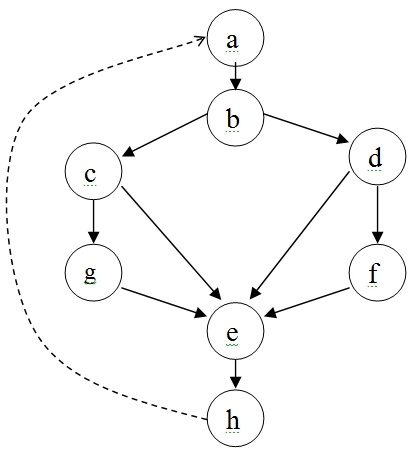
\includegraphics[width=11cm]{metrics_Mackkaib_1.jpg}
    \caption{граф в метриці Маккейба}
    \label{fig:awesome_image}
\end{figure}

Для програми цикломатичне число при l = 10, v = 8, n = 1 визначиться як Z ( G) = 10-8 +2 = 4 .

Таким чином, є Сільносвязанная граф з чотирма лінійно незалежними контурами :

a - b - c - g - e - h - a ;

a - b - c - e - h - a ;

a - b - d - f - e - h - a ;

a - b - d - e - h - a ;

Розглянемо метрику складності програми, що отримала назву « підрахунок точок перетину «, авторами якої є М Вудвард, М Хенель і Д Хидли . Метрика орієнтована на аналіз програм, при створенні яких використовувалося неструктурні кодування на таких мовах, як мова асемблера і фортран . Вводячи цю метрику, її автори прагнули оцінити взаємозв'язку між фізичними місцеположеннями керуючих переходів .

Структурний кодування припускає використання обмеженого безлічі керуючих структур в якості первинних елементів будь-якої програми . У класичному структурному кодуванні, що базується на роботах професора Ейндховенського технологічного університету ( Нідерланди ) Е. Дейкстри, оперують тільки трьома такими структурами : проходженням операторів, розвилкою з операторів, циклом над оператором. всі ці різновиди зображуються найпростішими планарними графами програм. За правилами структурного кодування будь-яка програма складається шляхом вибудовування ланцюжків з 3х згаданих структур або приміщення однієї структури в іншу. Ці операції не порушують планарности графа всієї програми .

У графі програми, де кожному оператору відповідає вершина, тобто не виключені лінійні ділянки, при передачі управління від вершини a до b номер оператора a дорівнює min ( a, b ), а номер оператора b - max ( a, b ) . Тоді перетин дуг з'являться, якщо

min ( a, b ) \textless{} min ( p, q ) \textless{} max ( a, b ) \& max ( p, q ) \textgreater{} max ( a, b ) \textbar{}

\begin{list}{0em}
\item[] Min ( a, b ) \textless{} max ( p, q ) \textless{} max ( a, b ) \& min ( p, q ) \textless{} min ( a, b ) .
\end{list}

Іншими словами, точка перетину дуг виникає у разі виходу управління за межі пари вершин ( a, b ).

Кількість точок перетину дуг графа програми дає характеристику неструктурованості програми.


\subsection{Метрика Джилба}
\label{2section:id12}
Однією з найбільш простих, але досить ефективних оцінок складності програм є метрика Т. Джилба, в якій логічна складність програми визначається як насиченість програми виразами IF\_THEN\_ELSE . При цьому вводяться дві характеристики :

СL - абсолютна складність програми, що характеризується кількістю операторів умови;
cl - відносна складність програми, що характеризується насиченістю програми операторами умови, тобто cl визначається як відношення CL до загального числа операторів.
Використовуючи метрику Джилба, її доповнили ще однією складовою, а саме характеристикою максимального рівня вкладеності оператора CLI, що дозволило застосувати метрику Джилба до аналізу циклічних конструкцій.

Великий інтерес представляє оцінка складності програм за методом граничних значень .

Введемо кілька додаткових понять, пов'язаних з графом програми .

Нехай G = (V, E) - орієнтований граф програми з єдиною початковою і єдиною окнечной вершинами. У цьому графі число входять до вершину дуг називається негативною ступенем вершини, а число що виходять з вершини дуг - позитивної ступенем вершини . Тоді набір вершин графа можна розбити на дві групи:

вершини у яких позитивна ступінь \textless{}= 1 ;
вершини у яких позитивна ступінь \textgreater{} = 2 .
Вершини першої групи назвемо приймаючими вершинами, а вершини другої групи - вершинами відбору.

Для отримання оцінки за методом граничних значень необхідно розбити

граф G на максимальне число подграфов G `, що задовольняють таким умовам:

вхід в подграф здійснюється тільки через вершину відбору;
кожен подграф включає вершину ( звану нижньою межею подграфа ), в яку можна потрапити з будь-якої іншої вершини подграфа . Наприклад, вершина відбору поєднана сама з собою дугою петлею, утворює подграф .

\begin{figure}
    \centering
    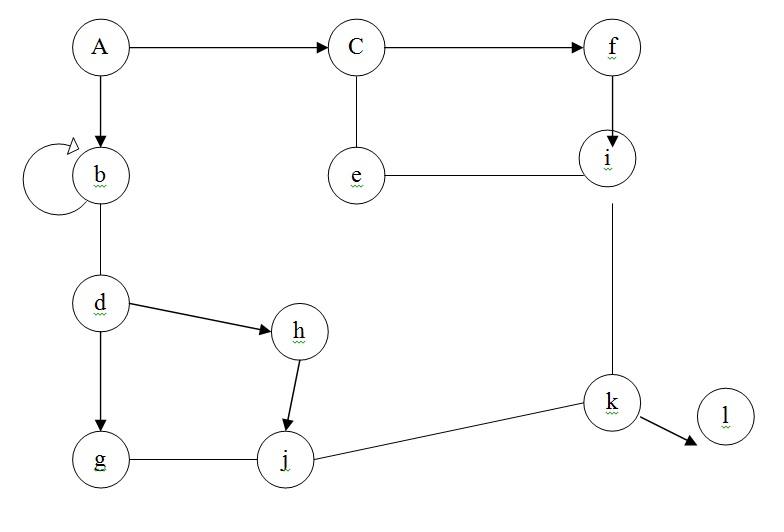
\includegraphics[width=15cm]{metrics_Jilb_1.jpg}
    \caption{граф в метриці Джилба}
    \label{fig:awesome_image}
\end{figure}

Число вершин, що утворюють такий подграф, одно скоригованої складності вершини відбору.

Кожна приймаюча вершина має скориговану складність, рівну 1, крім кінцевої вершини, скоригована складність якої дорівнює 0 . Скориговані складності всіх вершин графа G підсумовуються, утворюючи абсолютну граничну складність програми . Після цього визначається відносна гранична складність програми :

S0 = 1 - ( v - 1 ) / Sa,

де S0 - відносна гранична складність програми ; Sa - абсолютна гранична складність програми, v - загальне число вершин графа програми .

Таким чином, відносна складність програми дорівнює

S0 = 1 - ( 11 / 25 ) = 0,56 .

Інша група метрик складності програм - метрика складності потоку даних, тобто використання, конфігурації і розміщення даних в програмах.

Пара « модуль - глобальна змінна» позначається як ( p, r ), де p - модуль, що має доступ до глобальної змінної r . Залежно від наявності в програмі реального обігу до змінної r формуються два типи пар « модуль - глобальна змінна» : фактичні і можливі . Можливе звернення до r за допомогою p показує, що область існування r включає в себе p .

Характеристика Aup говорить про те, скільки разів модулі Up дійсно отримали доступ до глобальних змінних, а число Pup - скільки разів вони могли б отримати доступ.

Відношення числа фактичних звернень до можливих визначається

Rup = Aup / Pup

Ця формула показує наближену ймовірність посилання довільного модуля на довільну глобальну змінну. Очевидно, чим вище ця вірогідність, тим вище ймовірність « несанкціонованого » зміни якої-небудь змінної, що може істотно ускладнити роботи, пов'язані з модифікацією програми .

Покажемо розрахунок метрики « модуль - глобальна змінна» . Нехай у програмі є три глобальні змінні і три підпрограми. Якщо припустити, що кожна підпрограма має доступ до кожної з змінних, то ми отримаємо дев'ять можливих пар, тобто Pup = 9 . Далі нехай першим підпрограма звертається до однієї змінної, другий - двом, а третя не звертається ні до однієї змінної. Тоді Aup = 3, Rup = 3 /9.

\subsection{Алгоритм пошуку залежностей потенційно-небезпечних дефектів програм на основі екстраполяції метричних характеристик вихідних текстів програм для побудови дерева атак}
\label{2section:id13}

Розглянемо програмний продукт в якості множини вразливостей:

\begin{equation}
 Vuln = {Vuln_1,Vuln_2,....,Vuln_N}
\end{equation}

Маючи вищенаведені характеристики, та множину потенцыйних вразливостей пропоную створити наступну модель вибору потенційно небезпечних дефектів реакції програм для кібернетичного впливу:

\begin{equation}\label{eq:my_equation}
 P_{Vuln_i} = \frac{V_i Z(G)_i}{Z(G) \frac{V}{C_v}}Rup_i, 
\end{equation}
де

\begin{itemize}
\item {} 
V - Обсяг програми

\item {} 
Vi - обсяг підпрограми

\item {} 
Cv - кікькість потенційних вразливостей

\item {} 
Z(G)i - цикломатична складність підпрограми, в якій знаходиться дефект

\item {} 
Z(G) - цикломатична складність всього коду досліджуваного проекту

\item {} 
Rup - кількість звернень потенційно-вразливої ділянки коду до глобальних змінних

\end{itemize}

Розглянемо кожну властивість поданих метрик в контексті відображення наявності можливості використання дефекту переповнення буферу:
\begin{itemize}
\item {} 
Обсяг програми - обсяг програми напряму впливає на кількість помилок в ній

\item {} 
Аналогічним чиним від обсягу підпрограми, в якій знаходиться потенційна вразливість залежить можливість її використання

\item {} 
Від цикломатичної складності залежить наскільки просто буде проаналізувати логіку коду і швидко розібратись, як саме можна використати дефект

\item {} 
А від кількості звернень до потенційно-вразливої ділянки коду можна зробити висновок, як локальні дані між собою звязані і чи можливо здійснити вплив на певні управляючі дані через суміжні

\end{itemize}

Дана ймовірність буде наближеною та неточною, але якщо набір таких ймовірностей збільшувати і розглянути їх як протабульовану функцію
$f(V,V_i,C_v,Z(G)_i,Z(G),Rup) = P_{vuln_i}$
то можна спробувати робити прогноз наявності вразливих ділянок при аналізі нового вихідного тексту на основі  його метрик коду - що дозволить побудувати ефективне дерево атак.


\subsection{Дерева атак}
\label{2section:id14}
Дерева атак - це діаграми, що демонструють, як може бути атакована ціль. Дерева атак використовуються в безлічі областей. В області інформаційних технологій вони застосовуються, щоб описати потенційні загрози  у комп'ютерній системі і можливі способи атаки, які реалізують ці загрози. Однак, їх використання не обмежується аналізом звичайних інформаційних систем. Вони також широко використовуються в авіації і обороні для аналізу ймовірних загроз, пов'язаних зі стійкими до спотворень електронними системами.

Збільшується застосування дерев атак в комп'ютерних системах контролю (особливо пов'язаних з енергетичними мережами). Також дерева атаки використовуються для розуміння загроз, пов'язаних з фізичними системами.

Деякі з найбільш ранніх описів дерев атак знайдені в доповідях і статтях Брюса Шнайера, технічного директора Counterpane Internet Security. Шнайер був безпосередньо залучений в розробку концептуальної моделі дерев атаки і зіграв важливу роль в її поширенні. Тим не менш, в деяких ранніх опублікованих статтях по деревах атак висловлюються припущення про залученість Агентства Національної Безпеки в початковий етап розробки.

Дерева атак дуже схожі на дерева загроз. Дерева загроз були розглянуті в 1994 роки Едвардом Аморосо.

Дерева атак це мультирівневих діаграми, що складаються з одного кореня, листя і нащадків. Будемо розглядати вузли знизу вгору. Дочірні вузли це умови, які повинні виконуватися, щоб батьківський вузол також перейшов в справжній стан. Коли корінь переходить у справжній стан, атака успішно завершена. Кожен вузол може бути приведений у справжній стан тільки його прямими нащадками.

Вузол може бути дочірнім для іншого вузла, в цьому випадку, логічно, що для успіху атаки потрібно кілька кроків. Наприклад, уявіть клас з комп'ютерами, де комп'ютери прикріплені до парт. Щоб вкрасти один з них необхідно або перерізати кріплення, або відкрити замок. Замок можна відкрити відмичкою або ключем. Ключ можна отримати шляхом погроз його власнику, через підкуп власника або ж просто вкрасти його. Таким чином, можна намалювати чотирирівневої дерево атаки, де одним із шляхів буде: Підкуп власника ключа-Отримання ключа-Відмикання замку-Винос комп'ютера.

Також слід враховувати, що атака, описана у вузлі може зажадати, щоб одна або декілька з безлічі атак, описаних в дочірніх вузлах були успішно проведені. Вище ми показали дерево атаки тільки зі зв'язком типу АБО між нащадками вузла, але умова І також може бути введено, наприклад в класі є електронна сигналізація, яка повинна бути відключена, але тільки в тому випадку, якщо ми вирішимо перерізати кріплення. Замість того, щоб робити відключення сигналізації дочірнім вузлом для перерізання кріплення, обидва завдання можна просто логічно підсумувати, створивши шлях (Відключення сигналізації І Перерізання кріплення)-Винос Комп'ютера.

Дерева атак також пов'язані із створенням дерева помилок.  Метод побудови дерева помилок використовує булеві вирази для створення умов, при яких дочірні вузли забезпечують виконання батьківських вузлів.

Включає апріорні ймовірності в кожен вузол, можливо зробити підрахунок ймовірностей для вузлів, що знаходяться вище по правилу Байеса . Однак, в реальності, точні оцінки ймовірності або недоступні, або занадто дорогі для обчислення. У разі динамічної комп'ютерної безпеки (тобто з урахуванням атакуючих) випадкові події не є незалежними, отже, прямий Байєсівський аналіз не підходить.

Так як Байєсовські аналітичні техніки, що використовуються в аналізі дерев помилок не можуть бути правильно застосовані до дерев атак, аналітики використовують інші техніки для визначення яким шляхом піде даний атакуючий. Ці техніки включають порівняння можливостей атакуючого (час, гроші, навички, обладнання) з ресурсами, що вимагаються для даної атаки. Атаки, які вимагають повної віддачі від атакуючого або навіть знаходяться за межами його можливостей куди менш імовірні, ніж дешеві і прості атаки. Ступінь, в якій атака задовольняє цілям атакуючого також впливає на його вибір. З двох можливих атак зазвичай вибирається та, що більшою мірою задовольняє цілям атакуючого.

Дерева атак можуть стати вкрай складними, особливо при розгляді конкретних атак. Повне дерево атаки може містити сотні або тисячі різних шляхів, всі з яких призводять до успіху атаки. Але навіть при такому розкладі, ці дерева вкрай корисні для визначення існуючих загроз і методів їх запобігання.

Дерева атак можуть бути використані для визначення стратегії забезпечення інформаційної безпеки. Також, слід враховувати, що реалізація цієї стратегії сама по собі вносить зміни в дерево атаки. Наприклад, захистом від комп'ютерних вірусів може служити заборона системного адміністратора безпосередньо змінювати існуючі файли і папки, замість цього вимагаючи використання файлового менеджера. Це додає в дерево атаки використання недоліків чи експлойтів файлового менеджера.

\begin{figure}
    \centering
    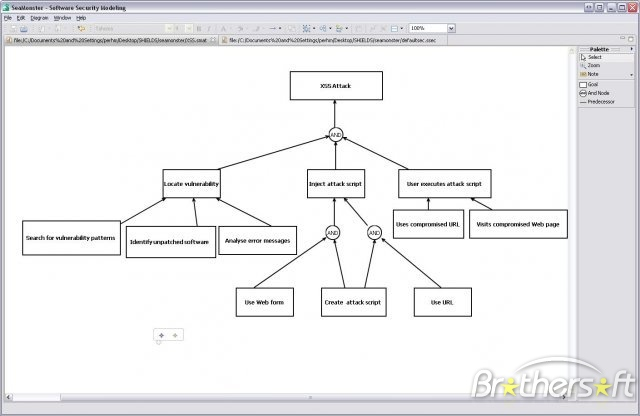
\includegraphics[width=15cm]{seamonster_attack_tree.jpeg}
    \caption{приклад дерева атак}
    \label{fig:attack_tree_example}
\end{figure}

\pagebreak

\section*{Висновки}
\addcontentsline{toc}{section}{Висновки}
Отже, проаналізувавши обчислення метрик інтегрованих властивостей вихідних кодів програмних засобів дозволяють зекономити час та інші ресурси в плані організації та розробки засобів кібернетичного впливу та побудови дерев атак тому підготовка фахівців в даній області є необхідною, як і розширення навчальної бази для досягнення даної цілі – на даний момент напрацьована невелика науково-методична база в даній області.

\chapter{ПРОГРАМНИЙ МОДУЛЬ ВИЗНАЧЕННЯ МЕТРИК ЦІЛЬОВОЇ ПРОГРАМИ ДЛЯ ПІДВИЩЕННЯ ЕФЕКТИВНОСТІ ДОСЛІДЖЕННЯ ЇЇ ПОТЕНЦІЙНО-НЕБЕЗПЕЧНИХ ДЕФЕКТІВ}
\label{3section::doc}\label{3section:id1}

\section{Структурна схема алгоритму та основні функціональні елементи}
\label{3section:id2}
Підчас аналізу предметної області мною була запропонована структурна схема програмно-технічного комплексу дослідження цільових програм на переповнення буфера 
\begin{figure} [h]
    \centering
    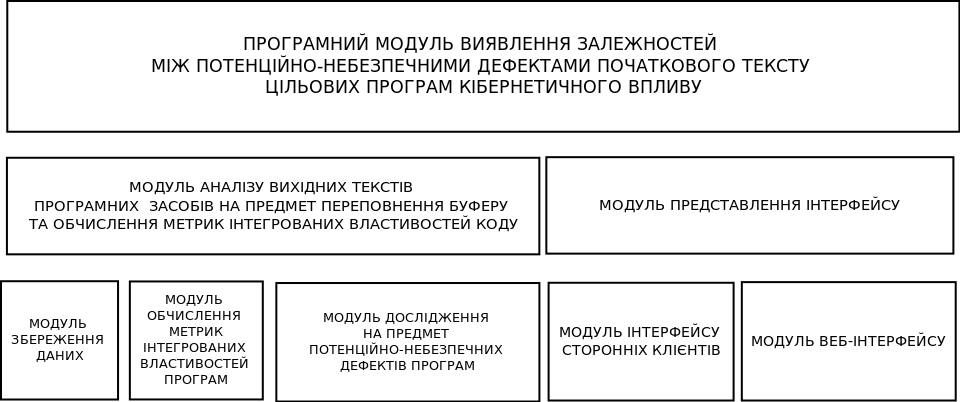
\includegraphics[width=16cm]{general_structure.png}
    \caption{Структурна схема модулю визначення метрик цільової програми}
    \label{fig:general_structure}
\end{figure}
(Рис \,\ref{fig:general_structure})

\section{Інтерфейс користувача}
\label{3section:id3}

\section{Керівництво щодо розгортання та експлуатації}
\label{3section:id4}

\section*{Висновки}
\addcontentsline{toc}{section}{Висновки}
Отже,


\chapter{ОЦІНКА ЕФЕКТИВНОСТІ ВИРІШЕННЯ ЗАДАЧІ ВИЯВЛЕННЯ ЗАЛЕЖНОСТЕЙ МІЖ ПОТЕНЦІЙНО-НЕБЕЗПЕЧНИМИ ДЕФЕКТАМИ ПОЧАТКОВОГО ТЕКСТУ ЦІЛЬОВИХ ПРОГРАМ КІБЕРНЕТИЧНОГО ВПЛИВУ}
\label{4section::doc}\label{4section:id1}

\section{Опис випробування та порівняльний аналіз результатів}
\label{4section:id2}

\section{Напрямки удосконалення прототипу системи}
\label{4section:id3}

\section*{Висновки}
\addcontentsline{toc}{section}{Висновки}
Отже,


\section*{ЗАКЛЮЧЕННЯ}
\addcontentsline{toc}{chapter}{ЗАКЛЮЧЕННЯ}
\label{5decision::doc}\label{5decision:id1}

\pagebreak

\section*{СПИСОК ВИКОРИСТАНОЇ ЛІТЕРАТУРИ}
\addcontentsline{toc}{chapter}{СПИСОК ВИКОРИСТАНОЇ ЛІТЕРАТУРИ}
\label{6literature::doc}\label{6literature:id1}\begin{enumerate}
\item {} 
\href{http://dorlov.blogspot.com/2009/11/blog-post.html}{http://dorlov.blogspot.com/2009/11/blog-post.html}

\end{enumerate}

\pagebreak

\section*{ДОДАТКИ}
\label{7addition::doc}\label{7addition:id1}
\addcontentsline{toc}{chapter}{ДОДАТКИ}

%\renewcommand{\indexname}{Індекс}
%\printindex
\end{document}
